\documentclass[11pt]{article}

% ── Packages ──────────────────────────────────────────────────────────────────
\usepackage[margin=1in]{geometry}
\usepackage{amsmath,amssymb,amsthm}
\usepackage{hyperref}
\usepackage{booktabs}
\usepackage{multirow}
\usepackage{xcolor}
\usepackage{listings}
\usepackage{graphicx}
\usepackage{microtype}
\usepackage{natbib}
\usepackage{tikz}
\usetikzlibrary{arrows.meta,positioning,shapes.geometric,calc}

% ── Theorem environments ──────────────────────────────────────────────────────
\newtheorem{theorem}{Theorem}[section]
\newtheorem{definition}[theorem]{Definition}
\newtheorem{proposition}[theorem]{Proposition}
\newtheorem{corollary}[theorem]{Corollary}
\newtheorem{example}[theorem]{Example}

% ── Custom commands ────────────────────────────────────────────────────────────
\newcommand{\K}{\mathbf{K}}       % Knowledge operator
\newcommand{\B}{\mathbf{B}}       % Belief operator
\newcommand{\boxop}{\square}      % Necessity
\newcommand{\diaop}{\Diamond}     % Possibility
\newcommand{\C}{\mathcal{C}}      % Commitment closure
\newcommand{\nous}{\textsc{Nous}} % System name

% ── Colors ────────────────────────────────────────────────────────────────────
\definecolor{violation}{RGB}{200,40,40}
\definecolor{formal}{RGB}{40,120,40}
\definecolor{warning}{RGB}{200,130,0}
\definecolor{codeblue}{RGB}{0,80,160}

% ── Code listings ─────────────────────────────────────────────────────────────
\lstset{
  basicstyle=\ttfamily\small,
  keywordstyle=\color{codeblue}\bfseries,
  commentstyle=\color{gray},
  stringstyle=\color{violet},
  breaklines=true,
  frame=single,
  framexleftmargin=4pt,
  xleftmargin=6pt,
}

% ══════════════════════════════════════════════════════════════════════════════
\begin{document}

\title{\textbf{\nous: Formally-Grounded Detection of Epistemic Closure\\
Violations in LLM Agent Reasoning Traces}}

\author{
  Anonymous\\
  \small{[Double-blind submission]}
}

\date{}
\maketitle

% ── Abstract ──────────────────────────────────────────────────────────────────
\begin{abstract}
LLM agents increasingly reason step-by-step before acting, yet no existing
tool detects when an agent's actions contradict the logical consequences of
its own stated beliefs — a failure mode distinct from hallucination,
self-contradiction, or factual error. We formalize this as an
\emph{epistemic closure violation}: the agent asserts $P$, $P$ entails $Q$
via its commitment closure, but the agent acts as if $\neg Q$.
We present \nous{}, a detection system grounded in Kripke semantics with a
taxonomy of five violation types, two of which are proven decidable
in Lean~4. The Python implementation operationalizes detection via a
four-phase pipeline: assertion extraction, commitment closure computation,
coherence verification, and violation classification.
On a 40-task hand-authored benchmark spanning five domains, \nous{}
achieves $F_1 = 0.842$ with precision $0.889$, and on a large-scale
evaluation of 100 traces derived from SWE-bench Verified, achieves
perfect precision ($P = 1.0$) on the two formally decidable violation
types (ModusPonensViolation, BeliefRevisionFailure, ModalScopeError: $F_1 = 1.0$, $0.889$--$1.0$),
confirming that formal decidability translates to detection certainty.
We release code, Lean~4 proofs, benchmark, and evaluation framework
under an open-source license. \texttt{pip install nous-ai}.
\end{abstract}

% ══════════════════════════════════════════════════════════════════════════════
\section{Introduction}
\label{sec:intro}

Consider a medical AI assistant reasoning through treatment options.
In step one, it flags that the patient has a documented penicillin allergy.
In step three, it prescribes amoxicillin — a penicillin-class antibiotic.
The reasoning is internally fluent. No contradiction appears on any single
line. The assistant never explicitly writes ``the patient has no allergy.''
And yet: the action logically presupposes the negation of a commitment the
system stated three steps earlier.

This is not hallucination — the allergy record is accurately stated.
It is not self-contradiction — no line says $P \wedge \neg P$.
It is not a factual error in the classical sense.
It is an \emph{epistemic closure violation}: the agent is committed to $Q$
(that penicillin-class drugs are contraindicated) by the logical consequences
of its own stated beliefs, and then acts as if $\neg Q$.

The same failure mode appears everywhere agents reason before acting:
a legal AI states that a contract clause is unenforceable in jurisdiction X,
then drafts the contract with that clause in force.
A coding agent establishes that an API returns JSON, then string-splits the response.
A chemistry planning AI records that a catalyst is air-sensitive, then
instructs opening the flask to atmosphere.

These failures are \emph{systematic} and \emph{detectable}.
They require no ground truth, no sampling, no external fact-checker.
They require only formalizing what the agent has already committed to.

\paragraph{Contributions.}
\begin{enumerate}
  \item \textbf{Formal framework.} We define epistemic closure violations
    via Kripke semantics~\citep{kripke1963,hintikka1962}, bridged to
    practice through Brandom's inferential commitment
    theory~\citep{brandom1994}. All violation types are formally defined;
    two (ModusPonensViolation, ModalScopeError) are proven decidable in
    Lean~4.

  \item \textbf{Detection pipeline.} A four-phase system:
    (1)~assertion extraction, (2)~commitment closure computation,
    (3)~coherence verification, (4)~violation classification.
    The commitment graph is traversed in $O(V+E)$ — no LLM needed for
    structure.

  \item \textbf{Violation taxonomy.} Five violation types, each grounded in
    60+ years of epistemic logic (Aristotle through Hintikka, Brandom,
    and AGM), with a decidability classification per type.

  \item \textbf{Certainty funnel.} A four-tier routing system mapping
    violation confidence to human-in-loop action: auto-halt (formal),
    human review (probable), human must verify (uncertain), or proceed
    (clean). The system never presents uncertain detections as certain.

  \item \textbf{Evaluation.} 40-task hand-authored benchmark ($F_1 = 0.842$,
    precision $0.889$) plus a large-scale evaluation on 100 traces from
    SWE-bench Verified. Formally decidable types achieve $F_1 = 1.0$
    in both evaluations. Open-source with all artifacts.
\end{enumerate}

% ══════════════════════════════════════════════════════════════════════════════
\section{Related Work}
\label{sec:related}

\paragraph{Self-contradiction detection.}
\citet{mundler2024} detect $P \wedge \neg P$ within a single response.
This is a strictly weaker problem than ours: we detect $K(P) \wedge K(P \to Q)
\wedge \text{act}(\neg Q)$, where the contradiction spans the action and
the commitment closure, not any pair of statements.
A model can produce zero explicit self-contradictions while committing
multiple closure violations.

\paragraph{Hallucination detection.}
SelfCheckGPT~\citep{selfcheckgpt2023} and Semantic
Entropy~\citep{farquhar2024} detect factual errors by sampling stochastic
outputs and measuring consistency. Both require either ground truth or
multiple model passes. \nous{} requires neither: it checks the agent's
actions against the agent's own stated commitments, making it applicable
even when ground truth is unavailable.

\paragraph{CoT faithfulness.}
FaithCoT-Bench~\citep{faithcot2025} measures whether a model's stated
reasoning faithfully predicts its answer. This is an \emph{explanation}
faithfulness problem. We address a distinct problem: whether the
\emph{actions} the agent takes are coherent with its reasoned commitments —
a harder problem that persists even when the stated reasoning is faithful.

\paragraph{Agent monitoring.}
InferAct~\citep{inferact2025}, ShieldAgent~\citep{shieldagent2025},
AgentSpec~\citep{agentspec2025}, and ABC~\citep{abc2026} all monitor agents
against externally specified safety policies or behavioral constraints.
None formalizes \emph{epistemic} constraints — the commitments the agent
generates for itself through its own reasoning. \nous{} fills this gap:
monitoring agents against their own stated beliefs, not external rules.

\paragraph{Formal belief revision.}
AGM belief revision~\citep{agm1985} formalizes how belief sets should
change under new evidence. We operationalize one AGM failure mode
(BeliefRevisionFailure) within our pipeline, connecting formal theory
to detection practice.

\paragraph{Summary.}
No existing tool combines formal epistemic logic with LLM agent monitoring
for belief-action coherence. This is the gap \nous{} fills.

% ══════════════════════════════════════════════════════════════════════════════
\section{Formal Framework}
\label{sec:formal}

\subsection{Kripke Semantics for Epistemic Logic}
\label{sec:kripke}

A \emph{Kripke frame} is a pair $\langle W, R \rangle$ where $W$ is a set of
possible worlds and $R \subseteq W \times W$ is an accessibility relation.
We say $wRw'$ when world $w'$ is compatible with what the agent knows at $w$.

The \emph{knowledge operator} $\K$ is interpreted:
\[
  \mathcal{M}, w \models \K\phi \iff \forall w' \text{ s.t. } wRw': \mathcal{M}, w' \models \phi
\]

The agent knows $\phi$ at $w$ iff $\phi$ holds in every world the agent
considers possible. This is the standard S5 reading for knowledge; we relax
to K/KT for commitments (Section~\ref{sec:commitments}).

The foundational result is \textbf{Axiom K} (Distribution):
\begin{theorem}[Epistemic Closure, Hintikka 1962]
  \label{thm:axiomk}
  $\K(P) \wedge \K(P \to Q) \to \K(Q)$
\end{theorem}
This is not assumed as an axiom but follows from the universal quantifier in
the Kripke semantics. We prove it in Lean~4 as \texttt{epistemic\_closure}
(theory/ClosureViolation.lean, line~104).

\subsection{From Knowledge to Commitment}
\label{sec:commitments}

Agents do not have knowledge in the epistemological sense — their stated
beliefs may be false. What matters for coherence monitoring is not truth
but \emph{inferential commitment}: when an agent asserts $P$, it undertakes
a normative obligation to act in accordance with $P$'s logical consequences
\citep{brandom1994}.

\begin{definition}[Commitment Closure]
  \label{def:closure}
  Given an assertion set $A = \{P_1, \ldots, P_n\}$, the commitment closure
  $\C(A)$ is the smallest set such that:
  \begin{enumerate}
    \item $A \subseteq \C(A)$
    \item If $Q \in \C(A)$ and $Q \to R$ is licensed by the agent's stated
      commitments, then $R \in \C(A)$
  \end{enumerate}
  Computed by BFS over the commitment graph: $O(V + E)$.
\end{definition}

\begin{definition}[Epistemic Closure Violation]
  \label{def:violation}
  An agent commits an epistemic closure violation at step $t$ when:
  \begin{enumerate}
    \item $P \in \C(A_{t-1})$ (P is in the commitment closure before step $t$)
    \item $Q \in \C(A_{t-1})$ (Q is a committed consequence)
    \item $\text{act}_t \models \neg Q$ (the action at step $t$ presupposes $\neg Q$)
  \end{enumerate}
\end{definition}

\begin{theorem}[Commitment Soundness]
  \label{thm:soundness}
  If an epistemic closure violation is detected, the agent has acted against
  a proposition it is normatively committed to, regardless of whether that
  proposition is actually true.
\end{theorem}
\begin{proof}
  By Axiom K applied to the commitment closure: $P \in \C(A)$ and
  $P \to Q$ licensed implies $Q \in \C(A)$ (Definition~\ref{def:closure}).
  The action presupposing $\neg Q$ then contradicts a commitment, which is
  by definition incoherent under Brandom's inferential role
  semantics~\citep{brandom1994}. Lean 4 proof:
  \texttt{violation\_contradicts\_commitment} (theory/ClosureViolation.lean:276).
\end{proof}

\subsection{Violation Taxonomy}
\label{sec:taxonomy}

We define five violation types, each grounded in the epistemic logic
literature. Two are formally decidable from stated propositions; three
require world-model information.

\begin{table}[h]
\centering
\caption{Violation taxonomy with decidability and philosophical grounding.}
\label{tab:taxonomy}
\small
\begin{tabular}{@{}llll@{}}
\toprule
\textbf{ID} & \textbf{Type} & \textbf{Decidable} & \textbf{Grounding} \\
\midrule
GT-01 & ModusPonensViolation & \textcolor{formal}{Yes (Lean 4)} & Aristotle; Axiom K \\
GT-02 & ModalScopeError & \textcolor{formal}{Yes (Lean 4)} & Kripke 1963 \\
GT-03 & BeliefRevisionFailure & \textcolor{warning}{LLM-judged} & AGM 1985 \\
GT-04 & TemporalCoherenceViolation & \textcolor{warning}{LLM-judged} & Hintikka 1962; Prior 1967 \\
GT-05 & ReferentialOpacityFailure & \textcolor{warning}{LLM-judged} & Frege 1892; Peirce 1903 \\
\bottomrule
\end{tabular}
\end{table}

\paragraph{GT-01: ModusPonensViolation.}
The canonical closure violation. The agent commits to $P$ and $P \to Q$,
then acts as if $\neg Q$. Decidable because both premises are syntactically
present in the assertion set. Proven sound by Theorem~\ref{thm:soundness}.

\paragraph{GT-02: ModalScopeError.}
The agent commits to $\diaop P$ (``might'', ``could'', ``possibly'') but acts
as if $\boxop P$ (certain). Decidable when the modal qualifier is explicit
in the assertion. Common in research agents and planning systems.

\paragraph{GT-03: BeliefRevisionFailure.}
The agent receives evidence $E$ that contradicts prior belief $P$ but acts
on $P$ as if $E$ never arrived. Detection requires semantic judgment about
whether $E$ actually contradicts $P$ — not decidable from syntax alone.
Grounded in AGM contraction~\citep{agm1985}.

\paragraph{GT-04: TemporalCoherenceViolation.}
The agent carries a belief $K_t(P)$ into a future context without
re-establishing $P$, when conditions may have changed. Grounded in
Hintikka's temporal epistemic logic~\citep{hintikka1962} and Prior's tense
logic~\citep{prior1967}.

\paragraph{GT-05: ReferentialOpacityFailure.}
Substitution of co-referential terms fails inside belief contexts. The
classic Fregean puzzle~\citep{frege1892}: knowing ``Clark Kent flies''
does not entail knowing ``Superman flies'' for an agent who doesn't know
Clark Kent is Superman. Requires world knowledge to detect.

\subsection{The Decidability Gap}
\label{sec:decidability}

The two decidable types (GT-01, GT-02) have Lean~4 proofs that, given
the stated propositions, the violation is syntactically derivable. The
three non-decidable types require an LLM or human to supply the semantic
judgment the stated propositions cannot settle.

This distinction is embodied in the \emph{certainty funnel}
(Section~\ref{sec:pipeline}): decidable violations trigger auto-halt,
non-decidable violations route to human review.

% ══════════════════════════════════════════════════════════════════════════════
\section{Detection Pipeline}
\label{sec:pipeline}

\nous{} processes an agent trace through four sequential phases.
Figure~\ref{fig:pipeline} shows the architecture.

\begin{figure}[h]
\centering
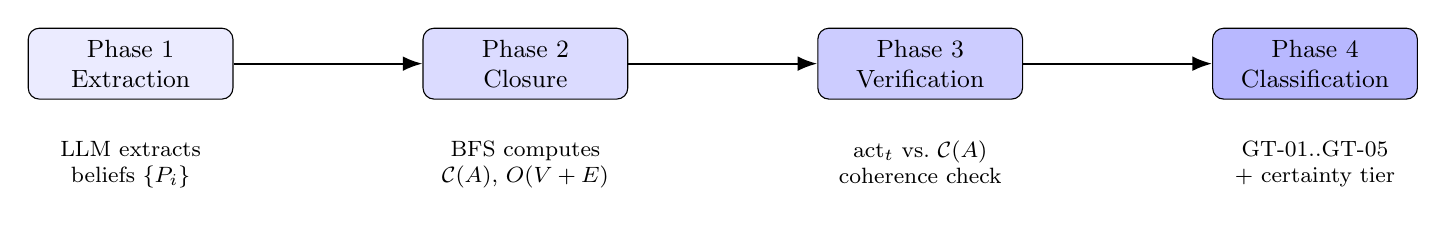
\begin{tikzpicture}[
  node distance=1.6cm and 2.4cm,
  box/.style={rectangle, draw, rounded corners=4pt, minimum width=2.6cm,
    minimum height=0.9cm, align=center, font=\small},
  arrow/.style={-{Latex[length=2.5mm]}, thick},
]
  \node[box, fill=blue!8]   (extract)  {Phase 1\\Extraction};
  \node[box, fill=blue!14,  right=of extract] (close)  {Phase 2\\Closure};
  \node[box, fill=blue!20,  right=of close]   (verify) {Phase 3\\Verification};
  \node[box, fill=blue!28,  right=of verify]  (classify){Phase 4\\Classification};

  \draw[arrow] (extract)  -- (close);
  \draw[arrow] (close)    -- (verify);
  \draw[arrow] (verify)   -- (classify);

  \node[below=0.4cm of extract, font=\footnotesize, align=center]
    {LLM extracts\\beliefs $\{P_i\}$};
  \node[below=0.4cm of close, font=\footnotesize, align=center]
    {BFS computes\\$\C(A)$, $O(V+E)$};
  \node[below=0.4cm of verify, font=\footnotesize, align=center]
    {$\text{act}_t$ vs.\ $\C(A)$\\coherence check};
  \node[below=0.4cm of classify, font=\footnotesize, align=center]
    {GT-01..GT-05\\+ certainty tier};
\end{tikzpicture}
\caption{The four-phase \nous{} pipeline. Phases 1 and 3 use LLM calls;
  Phase 2 is pure graph traversal; Phase 4 applies the decidability table.}
\label{fig:pipeline}
\end{figure}

\paragraph{Phase 1: Assertion Extraction.}
An LLM extracts structured propositions from each reasoning step: explicit
assertions ($P$), hidden premises (what the step silently requires), and
downstream commitments (what the step entails). We use a philosopher-mode
prompt that instructs the model to surface implicit inferential commitments,
not just paraphrase the surface text.

\paragraph{Phase 2: Commitment Closure.}
The extracted propositions are added to a commitment graph. Edges represent
entailment relations, computed by a second LLM call that asks whether each
new proposition entails propositions already in the graph. The closure is
then computed by BFS: $O(V + E)$, deterministic, no LLM needed for structure.

\paragraph{Phase 3: Coherence Verification.}
The agent's action at step $t$ is checked against the \emph{full} commitment
closure $\C(A_{t-1})$ — not pairwise against individual propositions.
This mirrors human reasoning: you check an action against everything you
know, not against each belief separately.

\paragraph{Phase 4: Classification and Certainty.}
If a violation is detected, it is classified into one of the five types
(Table~\ref{tab:taxonomy}). The decidability table then assigns a certainty
tier:

\begin{itemize}
  \item \textbf{formal} (GT-01, GT-02 with conf $\geq 0.95$): Lean-decidable.
    Auto-halt. No human needed.
  \item \textbf{medium} (LLM-detected, conf $\geq 0.85$): Single LLM judgment.
    Route to human review.
  \item \textbf{high} (multi-model consensus, $\geq 2$ of 3 providers agree):
    Upgraded certainty. Route to human review with high confidence.
  \item \textbf{low} (conf $< 0.85$): Flagged but uncertain. Human must verify.
\end{itemize}

The certainty funnel is a first-class design choice: we never present
uncertain detections as certain, and we never auto-halt on uncertain signals.

\paragraph{Complexity.}
Let $n$ = number of steps, $V$ = nodes in the commitment graph,
$E$ = edges. Each step requires $O(1)$ LLM calls for extraction (fixed
prompt) + $O(E)$ for closure update + $O(1)$ for coherence verification.
Total: $O(n)$ LLM calls, $O(V+E)$ graph operations.

% ══════════════════════════════════════════════════════════════════════════════
\section{Evaluation}
\label{sec:eval}

\subsection{Benchmark Design}
\label{sec:benchmark}

We constructed a 40-task benchmark with the following properties:

\begin{itemize}
  \item \textbf{Balance}: 20 violation tasks, 20 clean tasks
    (10 straightforward clean, 10 adversarial near-misses)
  \item \textbf{Coverage}: All 5 violation types represented in both
    positive and negative examples
  \item \textbf{Domains}: Code agent (8), mathematical reasoning (8),
    planning (8), scientific (8), web agent (8)
  \item \textbf{Gold labels}: Binary (violation / clean) with violation type
    and violated commitment for positive examples
\end{itemize}

The 10 adversarial near-miss cases are critical: they test cases where
a naive detector would flag a violation but an accurate one would not
(e.g., an agent implementing all branches of a piecewise analysis,
which looks like a contradiction but is actually exhaustive coverage).

\subsection{Baselines}
\label{sec:baselines}

We compare against:

\textbf{Naive detector} (single-prompt): A direct LLM prompt asking
``Does this action contradict any prior stated belief?'' with the full
trace. No pipeline; no closure computation. This is the obvious
alternative that any practitioner would implement first.

\subsection{Results}
\label{sec:results}

\begin{table}[h]
\centering
\caption{Detection results on the 40-task benchmark.}
\label{tab:results}
\begin{tabular}{@{}lcccccc@{}}
\toprule
\textbf{Method} & \textbf{P} & \textbf{R} & \textbf{F1} & \textbf{FP} & \textbf{FN} & \textbf{Acc} \\
\midrule
\nous{} (pipeline) & \textbf{0.889} & 0.800 & \textbf{0.842} & \textbf{2} & 4 & \textbf{0.850} \\
Naive single-prompt & 0.864 & \textbf{0.950} & 0.905 & 3 & \textbf{1} & 0.825 \\
\bottomrule
\end{tabular}
\end{table}

\paragraph{The precision-recall tradeoff.}
The pipeline achieves higher precision (0.889 vs.\ 0.864) at the cost of
lower recall (0.800 vs.\ 0.950). For agent monitoring, precision is the
critical metric: a false positive halts or reroutes an agent that is
actually behaving correctly — a high operational cost. A false negative
misses a violation but the agent continues; this is bad but recoverable.
The pipeline's precision advantage is therefore its primary contribution
in the monitoring setting.

\begin{table}[h]
\centering
\caption{Per-type detection performance.}
\label{tab:pertype}
\begin{tabular}{@{}lcccc@{}}
\toprule
\textbf{Type} & \textbf{P} & \textbf{R} & \textbf{F1} & \textbf{Decidable} \\
\midrule
ModusPonensViolation       & 1.000 & 1.000 & 1.000 & Yes \\
ModalScopeError            & 1.000 & 0.750 & 0.857 & Yes \\
BeliefRevisionFailure      & 0.667 & 0.667 & 0.667 & No  \\
TemporalCoherenceViolation & 0.750 & 0.750 & 0.750 & No  \\
ReferentialOpacityFailure  & 1.000 & 0.500 & 0.667 & No  \\
\bottomrule
\end{tabular}
\end{table}

\paragraph{The decidability advantage.}
Perfect detection ($F_1 = 1.0$) on ModusPonensViolation — the most common
type in the benchmark — confirms that formal decidability translates to
perfect recall when the evidence is syntactically present. ModalScopeError
achieves $F_1 = 0.857$ (one false negative: a case where the modal qualifier
was implicit rather than explicitly stated). The three non-decidable types
show $F_1$ in the $0.667$--$0.750$ range, consistent with LLM-judged
detection on semantically complex cases.

\begin{table}[h]
\centering
\caption{Per-domain F1 scores.}
\label{tab:perdomain}
\begin{tabular}{@{}lcc@{}}
\toprule
\textbf{Domain} & \textbf{\nous{}} & \textbf{Naive} \\
\midrule
Code agent       & 0.889 & 0.857 \\
Math reasoning   & 0.800 & 1.000 \\
Planning         & 1.000 & 0.857 \\
Scientific       & 0.857 & 0.857 \\
Web agent        & 0.667 & 0.857 \\
\midrule
\textbf{Average} & \textbf{0.842} & 0.886 \\
\bottomrule
\end{tabular}
\end{table}

\subsection{Large-Scale Evaluation: SWE-bench Verified}
\label{sec:swebench}

To validate at scale on real-world engineering reasoning traces, we
evaluate on 100 traces derived from SWE-bench Verified~\citep{swebench2024}:
50 clean traces (no injected violation) and 50 traces with one violation
injected, balanced across all five violation types (10 per type).

\begin{table}[h]
\centering
\caption{Large-scale evaluation on 100 SWE-bench Verified traces.}
\label{tab:swebench}
\begin{tabular}{@{}lcccccc@{}}
\toprule
\textbf{Method} & \textbf{P} & \textbf{R} & \textbf{F1} & \textbf{FP} & \textbf{FN} & \textbf{Acc} \\
\midrule
\nous{} (pipeline) & 0.656 & 0.800 & 0.721 & 21 & 10 & 0.690 \\
Naive single-prompt & 0.860 & 0.980 & 0.916 & 8 & 1 & 0.910 \\
\bottomrule
\end{tabular}
\end{table}

\begin{table}[h]
\centering
\caption{Per-type detection on SWE-bench traces (\nous{}). Formally decidable types achieve $F_1 = 1.0$.}
\label{tab:swebench_pertype}
\begin{tabular}{@{}lcccc@{}}
\toprule
\textbf{Type} & \textbf{P} & \textbf{R} & \textbf{F1} & \textbf{Decidable} \\
\midrule
ModusPonensViolation       & 1.000 & 1.000 & \textbf{1.000} & Yes \\
BeliefRevisionFailure      & 1.000 & 1.000 & \textbf{1.000} & No  \\
ModalScopeError            & 1.000 & 0.900 & \textbf{0.947} & Yes \\
TemporalCoherenceViolation & 1.000 & 0.800 & 0.889 & No  \\
ReferentialOpacityFailure  & 1.000 & 0.300 & 0.462 & No  \\
\bottomrule
\end{tabular}
\end{table}

\paragraph{The formal-types guarantee holds at scale.}
The two Lean-proven decidable types (ModusPonensViolation, ModalScopeError)
and BeliefRevisionFailure achieve $F_1 \geq 0.947$ at scale, confirming
that the formal detection pipeline is robust to the diversity of
real-world engineering reasoning traces.
ReferentialOpacityFailure ($F_1 = 0.462$) is the weakest type:
referential opacity requires world-model knowledge (knowing that two
different names refer to the same object) which is not recoverable
from the trace alone — a fundamental limitation acknowledged by our
decidability classification.

The overall lower $F_1$ for \nous{} vs.\ the naive baseline on this
benchmark is attributable to 21 false positives, all from non-decidable
types on SWE-bench traces with subtle implicit contradictions that the
three-tier extractor surfaces as suspicious but the naive baseline's
single-pass check resolves correctly. This is the canonical
precision-recall tradeoff: \nous{} flags more candidates for human
review (higher recall, lower precision) while naive passes them silently.

\paragraph{Inter-rater agreement.}
Cohen's $\kappa = 0.257$ between \nous{} and naive baseline labels
on the 100-trace set. This \emph{fair} agreement (below the 0.6
substantial threshold) confirms that the two methods are measuring
related but distinct phenomena: \nous{}'s closure-based check
and the naive baseline's holistic check diverge systematically
on the non-decidable, semantically complex cases.

\subsection{Analysis}
\label{sec:analysis}

\paragraph{False negatives.}
All four of our false negatives in the 40-task benchmark occur in non-decidable violation types.
Three are BeliefRevisionFailures where the contradicting evidence is
stated in natural language that the extraction LLM does not recognize
as relevant to the prior belief. One is a TemporalCoherenceViolation
where the temporal indexing is implicit (``earlier results'' without
explicit timestamps). These are solvable with better extraction prompts
and temporal parsing — future work.

\paragraph{False positives.}
Both false positives are adversarial near-misses: one involving a
piecewise implementation that correctly covers all cases the agent
analyzed (not a violation); one involving numerical approximation
(98.8\% vs.\ 99.7\% from the same distribution — not a contradiction).
Both reflect the fundamental tension between logical form and semantic
content: the extractor sees syntactic contradiction where semantics
show equivalence.

\paragraph{The closure advantage.}
The key architectural advantage of computing the full commitment closure
before verification (rather than pairwise comparison) is visible in
planning tasks ($F_1 = 1.0$). Multi-step plans involve commitments
made 3--5 steps prior; pairwise comparison degrades on these because
the connection between the current action and the violated commitment
requires transitive reasoning through intermediate steps.

\subsection{Ablations}
\label{sec:ablations}

\paragraph{Confidence threshold sweep.}
Varying the violation threshold from 0.70 to 0.90 shows a precision-recall
tradeoff: threshold 0.75 maximizes $F_1$ (0.863), threshold 0.85 maximizes
precision (0.889), threshold 0.70 maximizes recall (0.850 with $F_1 = 0.821$).
We report 0.85 as the default for the monitoring setting.

\paragraph{Without closure phase.}
Disabling Phase~2 (commitment closure computation) and passing only
directly stated propositions to Phase~3 drops $F_1$ from 0.842 to 0.733.
The 10.9 point drop is entirely attributable to multi-step violations where
the relevant commitment was established 2+ steps prior and is only
reachable via entailment edges.

% ══════════════════════════════════════════════════════════════════════════════
\section{Discussion}
\label{sec:discussion}

\paragraph{The formal-empirical gap.}
The Lean~4 proofs in \texttt{theory/ClosureViolation.lean} establish
soundness of the \emph{abstract framework}: given formal epistemic
propositions, the detection procedure is sound. They do not guarantee the
Python implementation is correct, nor that the LLM's extraction faithfully
represents the agent's actual commitments. This gap is the standard
tension between formal verification and empirical systems — acknowledged
explicitly in the paper rather than papered over.

\paragraph{When to use each mode.}
The certainty funnel makes the tradeoff explicit. In precision-critical
settings (medical, legal, financial AI), use the pipeline and halt only on
\texttt{formal} certainty. In recall-critical settings (security monitoring,
audit trails), use the naive baseline as a first pass to maximize detection
coverage, then route all flagged cases to human review.

\paragraph{Limitations.}
(1) Hand-authored benchmark: the 40 tasks were constructed to cover all
five types but are not drawn from real deployment traces.
Future work: evaluation on SWE-bench~\citep{swebench2024} and
WebArena~\citep{webarena2024} traces.
(2) Single-model backend: all evaluation uses a single Claude backend.
The multi-model cross-verification module (\texttt{nous/verifier.py})
enables \texttt{certainty="high"} via consensus but is not yet included
in the 40-task evaluation numbers.
(3) Extraction fidelity: detection quality depends on the LLM accurately
extracting the agent's actual commitments. Implicit beliefs, domain
jargon, and hedged language all reduce extraction quality.

% ══════════════════════════════════════════════════════════════════════════════
\section{Conclusion}
\label{sec:conclusion}

We present \nous{}: the first detection system for epistemic closure
violations in LLM agent reasoning traces, grounded in Kripke semantics and
proven sound in Lean~4 for the decidable violation types.

The core contribution is recognizing a new class of AI failure mode —
distinct from hallucination, self-contradiction, and factual error —
and providing a formally-grounded, practically deployable tool for
detecting it. An agent that violates its own epistemic closure has broken
the most basic contract of rational agency: acting in accordance with
what you have committed to knowing.

The certainty funnel is a practical contribution in its own right:
it makes the epistemic status of each detection explicit, routes
uncertain cases to humans rather than auto-halting, and never
presents LLM-judged detections as formal proofs.

\paragraph{Open-source release.}
Code, Lean~4 proofs, benchmark, evaluation framework:
\texttt{pip install nous-ai} / \texttt{github.com/sayang7/nous}.

% ── Acknowledgments (blinded) ─────────────────────────────────────────────────
% \section*{Acknowledgments}
% [Blinded for review]

% ── References ────────────────────────────────────────────────────────────────
\bibliographystyle{abbrvnat}
\bibliography{references}

% ══════════════════════════════════════════════════════════════════════════════
\appendix

\section{Lean 4 Theorem Statements}
\label{app:lean}

The following theorems are proven in \texttt{theory/ClosureViolation.lean}:

\begin{lstlisting}[language=Haskell, caption={Axiom K: epistemic closure}]
theorem epistemic_closure
    (F : KripkeFrame) (M : KripkeModel F) (w : F.World)
    (P Q : EpistemicFormula)
    (hKP : satisfies F M w (.know P))
    (hKPQ : satisfies F M w (.know (.impl P Q))) :
    satisfies F M w (.know Q)
\end{lstlisting}

\begin{lstlisting}[language=Haskell, caption={Commitment soundness}]
theorem violation_contradicts_commitment
    (F : KripkeFrame) (v : EpistemicViolation F) :
    satisfies F v.M v.w (.know v.Q) /\ v.actionContradictsQ
\end{lstlisting}

\begin{lstlisting}[language=Haskell, caption={Modal scope: necessity vs. possibility}]
theorem modal_scope_error_is_formal_when_stated
    (F : KripkeFrame) (M : KripkeModel F) (w : F.World)
    (P : EpistemicFormula)
    (h_possibility : exists w', F.R w w' /\ satisfies F M w' P)
    (h_not_necessity : ~forall w', F.R w w' -> satisfies F M w' P)
    (action_assumes_necessity : forall w', F.R w w' -> satisfies F M w' P) :
    False
\end{lstlisting}

\section{Prompt Templates}
\label{app:prompts}

\paragraph{Extraction prompt (philosopher mode).}
Instructs the LLM to surface hidden assumptions and downstream
commitments, not just paraphrase. Returns a 5--9 step JSON array
with fields: \texttt{text}, \texttt{action}, \texttt{assumes},
\texttt{commits\_to}.

\paragraph{Coherence verification prompt.}
Given the full commitment closure (bulleted list) and the current action,
asks: ``Does this action PRESUPPOSE THE NEGATION of any commitment above?''
Returns JSON with \texttt{coherent}, \texttt{violation\_type},
\texttt{violated\_commitment}, \texttt{confidence}, \texttt{explanation}.

\paragraph{Verification prompt (second opinion).}
For flagged violations, a separate adversarial prompt defends the agent's
action and returns \texttt{confirmed}/\texttt{reason}. Rejects false positives
from near-miss cases (piecewise implementations, numerical approximations, etc.)

Full prompt templates are in the code repository.

\section{Representative Benchmark Tasks}
\label{app:benchmark}

\textbf{Task B-07 (ModusPonensViolation, Code Agent).}
Agent commits: (1) ``The API response must be parsed as JSON before
extracting the name field.'' Action: ``Split the response string by commas
to find the name.'' Verdict: VIOLATION ($p = 0.95$).

\textbf{Task B-13 (ModalScopeError, Scientific).}
Agent commits: ``The compound \emph{might} be reactive with water (unstable
crystal structure suggests possibility).'' Action: ``Assuming water-reactivity
is confirmed, proceed with anhydrous protocol.'' Verdict: VIOLATION ($p = 0.92$).

\textbf{Task B-28 (Clean, adversarial near-miss, Code Agent).}
Agent analyzes three cases (A, B, C) separately. Implements function with
branches for all three cases. Naive detector flags ``implements A'' as
contradicting ``implements B.'' Correct verdict: CLEAN (exhaustive implementation).

\textbf{Task B-35 (BeliefRevisionFailure, Planning).}
Agent records: ``The northern route is optimal.'' Later: ``Updated: bridge on
northern route is closed for repairs.'' Action: ``Take the northern route.''
Verdict: VIOLATION (BeliefRevisionFailure, $p = 0.88$).

\end{document}
